\section{Architektur}

Dieses Kapitel erläutert den Aufbau unserer Applikation.
Auf der Abbildung \ref{fig:overview} sind die wichtigsten Klassen und Interfaces der Applikation ersichtlich. In der Tabelle \ref{tab:class} sind
die wichtigsten Klassen beschrieben.

\begin{figure}[ht]
	\begin{center}
		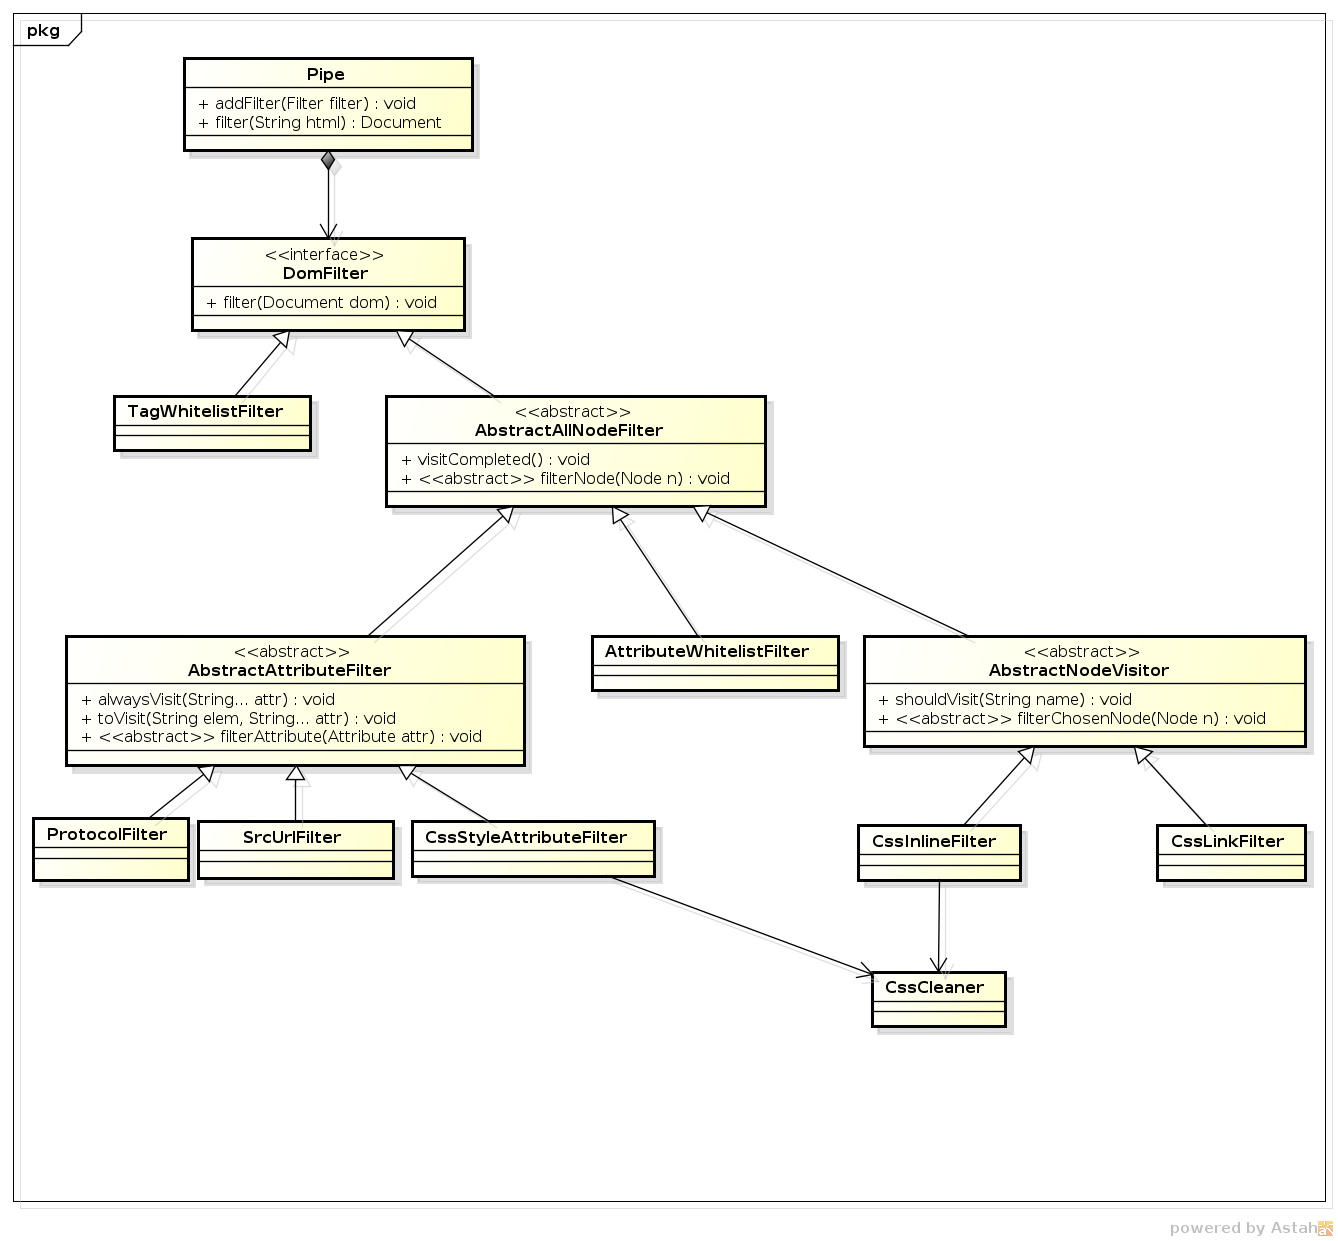
\includegraphics[width=1.0\textwidth]{./content/Class_Overview.png}
	\end{center}
	\caption{Übersicht über die Klassen und Interfaces}
	\label{fig:overview}
\end{figure}

\begin{table}[H]
\begin{center}
\begin{tabular}{l p{10.5cm} }
\hline
\textbf{Klasse} & \textbf{Beschreibung} \\ \hline \hline
Server      & Einstiegspunkt in die Applikation. Verwendet den Java HttpServer (com.sun.net.httpserver). Registiert die HttpHandler und startet den HttpServer. 
              Erstellt beim Start einen neuen User- und SessionManager. \\
XYHandler   & Nehmen HTTP Anfragen auf einer bestimmten URL entgegen und geben eine HTTP-Respone zurück. \\
UserManager & Verwaltet die Benutzer. Validiert beim Erstellen eines Benutzers den Benutzername und die E-Mail Adresse mit Hilfe der Klasse UserValidator.
              Wirft eine Exception, wenn der Benutzer nicht erstellt werden kann. \\
SessionManager & Verwaltet die ClientSessions. Ordnet jeder Session ein Token zu, mit welchem die Session identifiziert werden kann. \\
\hline \hline
\end{tabular}
\caption{Klassen}
\label{tab:class}
\end{center}
\end{table}

\begin{table}[H]
\begin{center}
\begin{tabular}{l l p{7cm} }
\hline
\textbf{Pfad} & \textbf{Handler}    & \textbf{Beschreibung} \\ \hline \hline
/             & WelcomeHandler          & Stellt die Loginseite index.html dar.\\
/register     & RegistrationHandler     & Verarbeitet die Registierungsanfrage und zeigt, wenn die Registierung erfoglreich war, einen Link zum Secure Content an. \\
/secured      & SecuredContentHandler   & Stellt wenn der Benutzer erfoglreich authentifiziert ist den Secure Content dar.\\
\hline \hline
\end{tabular}
\caption{URL-Mapping}
\label{tab:url-mapping}
\end{center}
\end{table}

\subsection{Authentifizierungsablauf}

Das Aktivitätsdiagramm Abbildung \ref{fig:process} beschreibt den Loginprozess bei einer HTTP-POST Anfrage auf /register mit einem gültigen Benutzernamen und E-Mail Adresse.
Als Resultat wird eine HTTP-Respone zurückgegeben, welche ein Cookie mit der Token ID setzt.

\begin{figure}[H]
	\begin{center}
		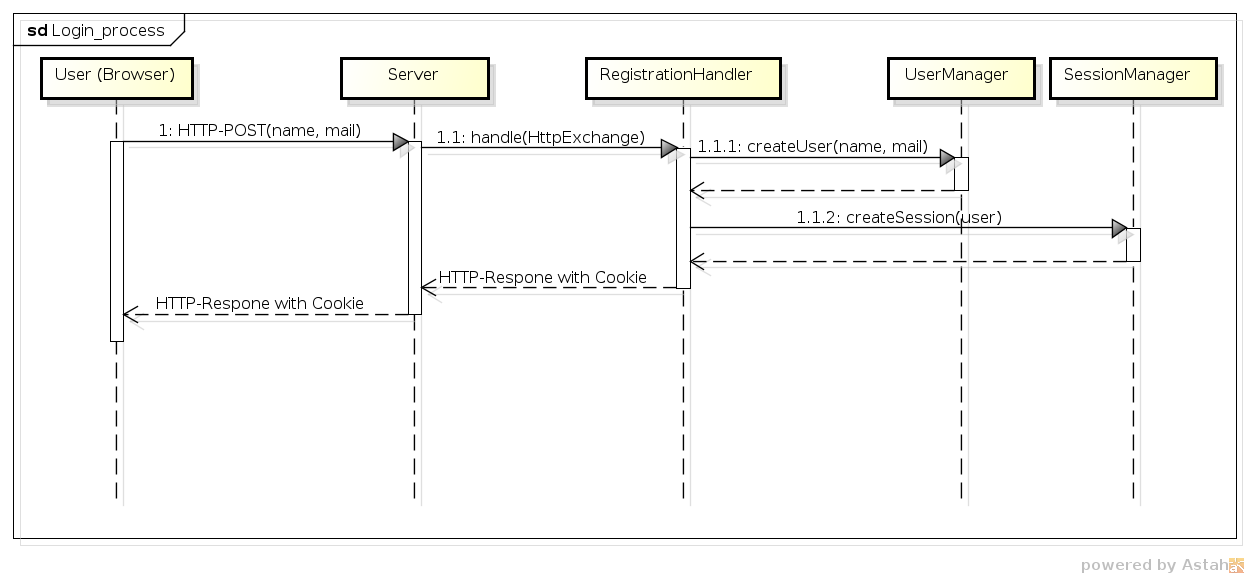
\includegraphics[width=1.0\textwidth]{./content/Login_process.png}
	\end{center}
	\caption{Loginprozess}
	\label{fig:process}
\end{figure}
